% %% %%%%%%%%%%%%%%%%%%%%%%%%%%%%%%%%%%%%%%%%%%%%%%%%%%%%%%%%%%
% step-6.tex
%
% Author:  Mauricio Matamoros
% License: MIT
%
% %% %%%%%%%%%%%%%%%%%%%%%%%%%%%%%%%%%%%%%%%%%%%%%%%%%%%%%%%%%%

%!TEX root = ../practica.tex
%!TEX root = ../references.bib

% CHKTEX-FILE 1
% CHKTEX-FILE 13
% CHKTEX-FILE 46

\subsection{Paso 6: Grabación y prueba}%
\label{sec:step6}
Una vez que el sistema termine de compilar, encontrará la imagen generada \texttt{.img} dentro del directorio \texttt{output/images} de \emph{buldroot}.
Notará que el archivo de imagen no pesa más de 300MB.
¡Así de pequeño es su sistema operativo embebido!

Proceda a grabar la imagen generada en una memoria microSD utilizando \href{https://etcher.balena.io/}{Balena Etcher} de la misma forma que ha grabado otras imágenes.
Alternativamente puede grabar la imagen utilizando \texttt{dd} si conoce la ruta de la misma en su sistema con el comando:

\begin{Verbatim}[gobble=1]
	# dd if=output/images/sdcard.img of=/dev/<memoriaSD> bs=10M status=progress
\end{Verbatim}

\noindent
La grabación no debería tomar más que unos segundos.

% \begin{wrapfigure}{r}{0.4\textwidth}
% 	\centering
% 	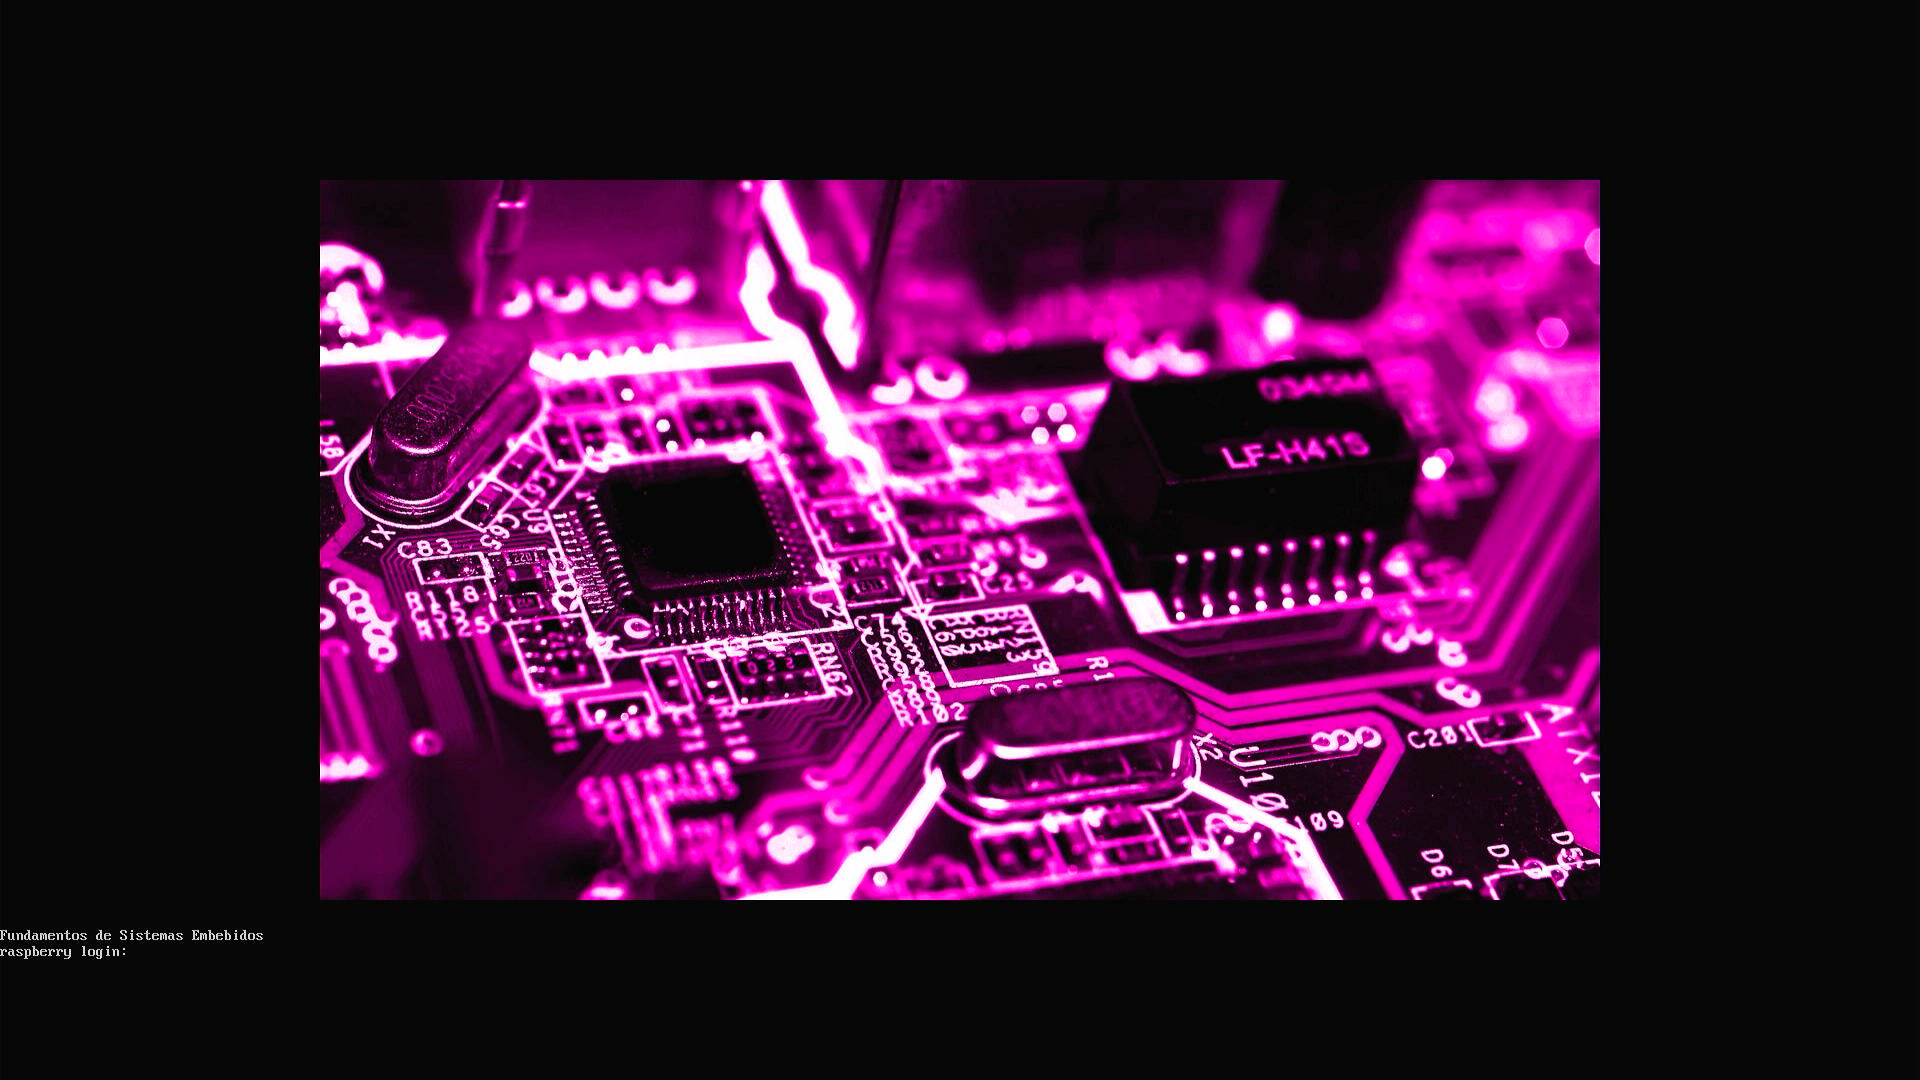
\includegraphics[width=0.38\textwidth]{img/system-running.jpg}
% \end{wrapfigure}
\begin{figure}
	\centering
	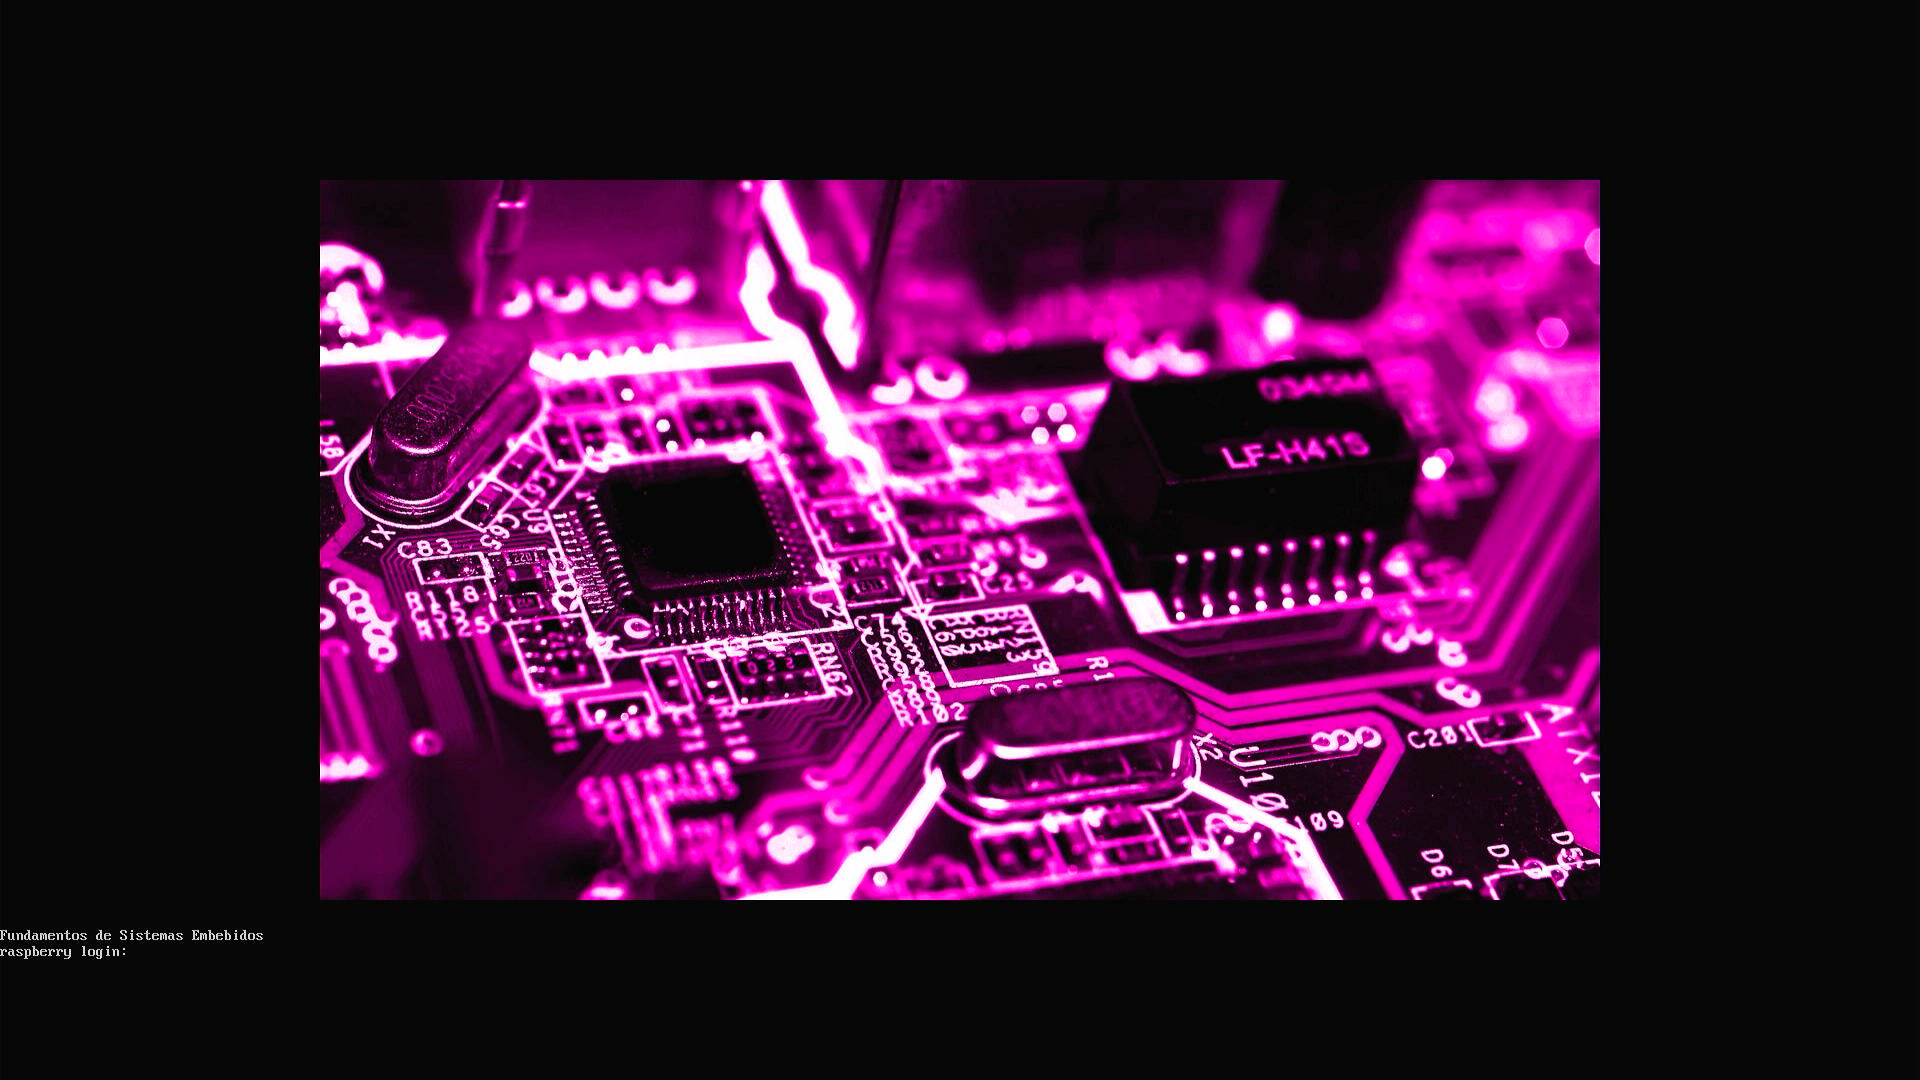
\includegraphics[width=0.8\textwidth,height=7cm,keepaspectratio]{img/system-running.jpg}
	\caption{Sistema embebido en ejecución con logotipo personalizado}%
	\label{fig:system-running}
\end{figure}
\medskip{}

Terminada la grabación, inserte la memoria microSD en la Raspberry Pi y observe el proceso de arranque, tendría que ver una pantalla similar a la de la~\Cref{fig:system-running}.
Cuando se lo solicite, inicie sesión con el usuario \texttt{pi} y la contraseña \texttt{raspberry}.


Conecte el display al puerto \IIC{} (pines 3 y 5 del puerto o GPIO2 y GPIO3 en BCM) y ejecute el comando de detección de dispositivos

\begin{Verbatim}[gobble=1]
	$ i2cdetect -y 1
\end{Verbatim}

\noindent
tendría que ver una salida como la siguiente:

\begin{Verbatim}[gobble=1]
	$ i2cdetect -y 1
	     0  1  2  3  4  5  6  7  8  9  a  b  c  d  e  f
	00:          -- -- -- -- -- -- -- -- -- -- -- -- --
	10: -- -- -- -- -- -- -- -- -- -- -- -- -- -- -- --
	20: -- -- -- -- -- -- -- 27 -- -- -- -- -- -- -- --
	30: -- -- -- -- -- -- -- -- -- -- -- -- -- -- -- --
	40: -- -- -- -- -- -- -- -- -- -- -- -- -- -- -- --
	50: -- -- -- -- -- -- -- -- -- -- -- -- -- -- -- --
	60: -- -- -- -- -- -- -- -- -- -- -- -- -- -- -- --
	70: -- -- -- -- -- -- -- --
\end{Verbatim}
